\documentclass[11pt]{article}
\usepackage{amsmath,textcomp,amssymb,geometry,graphicx}
\author{Ben Augarten}
\title{CS 189: HW6 Report}
\begin{document}
\maketitle
\section{Eigenfaces}
\begin{enumerate}
\item
The variations correspond to facial hair, hair, gender, skin color, eye color, hair color, lighting, smile type and eye positioning/wrinkles. You can visualize these by running visualize\_eigenfaces()
\item
To visualize the faces side by side using 10 eigenfaces, run
compare\_faces(index), where index is the ith celebrity face to reconstruct

Note, I didn't have very much success with 10 eigenfaces. I found that using more around 50 produced better results in reconstruction.\\
You can change this number within the compare\_faces function, just pass another parameter,\\
compare\_faces(index, num\_eigenfaces)

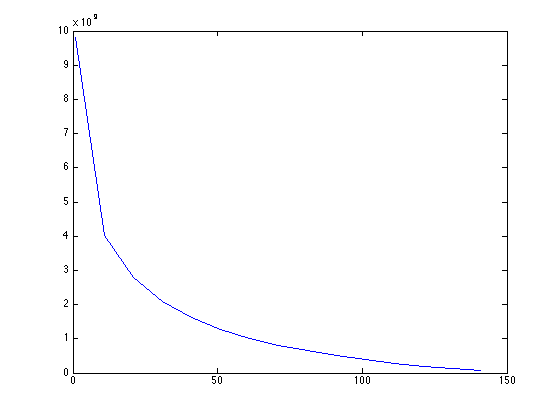
\includegraphics[width=\textwidth,height=3in]{L_2_err.png}

\item
To find the closest celebrity faces using euclidean distance, simply run\\
euclidean\_dist(i, true)\\
aka euclidean\_dist(5, true)\\

where i is the ith student\_image\\
true sets the function to display the images, otherwise it just returns the row vectors of the celebrities

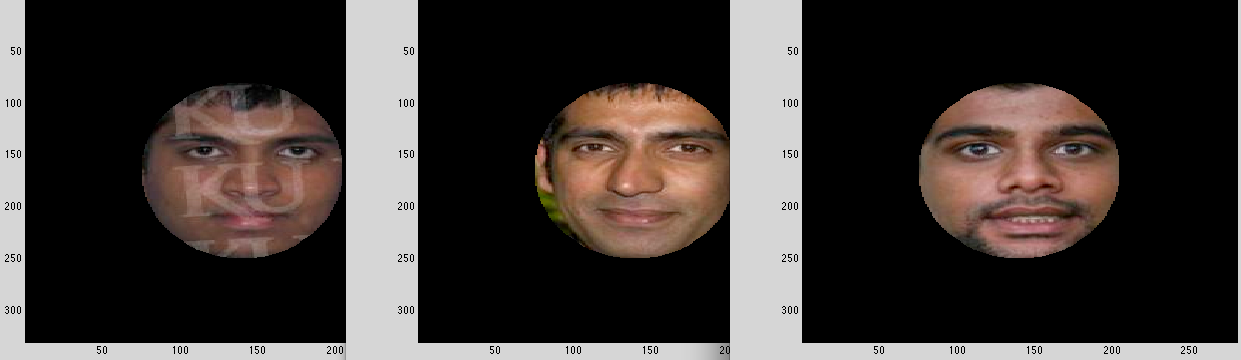
\includegraphics[width=\textwidth,height=3in]{euclidean_dist_1.png}

\item
We can use the matrix of eigenvalues as our $\Sigma$ because, obvious there exists a decomposition of $X=U\Sigma V^T$. Of course, this isn't in our eigenface basis. So we can preform a change of basis into eigenface coordinates. This change of basis will affect the eigenvectors but not the eigenvalues, aka $\Sigma$ will stay the same, so we can use $\Sigma$ as our $\Sigma$ when computing the Mahalanobis distance.\\

The display the student and nearest celebrity faces next to each other, simply run \\

mahalanobis\_distance(i, true)\\
aka: mahalanobis\_distance(5, true)\\
where i is the ith student\_image \\
true sets the function to display the image, rather than return the celebrities.\\
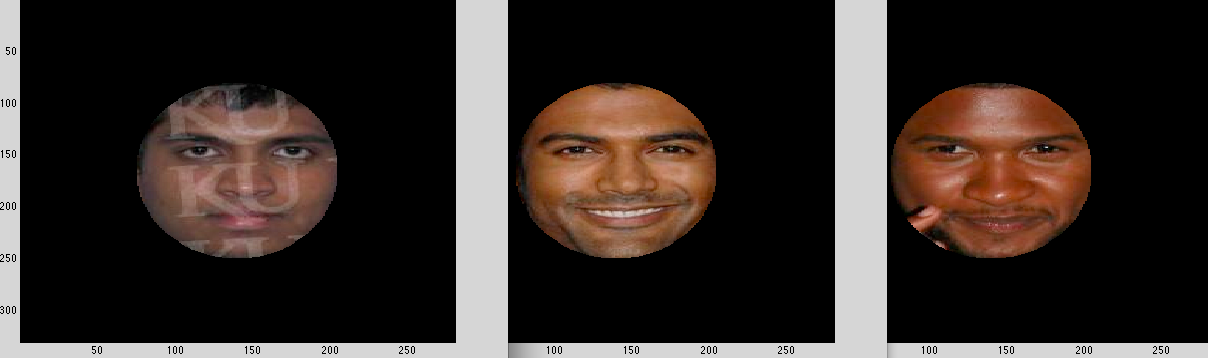
\includegraphics[width=\textwidth,height=3in]{mahalanobis_dist_1.png}
\end{enumerate}
\section{SVD}
\begin{enumerate}
\item
$AA^T=\begin{pmatrix} 2 & 2 \\ 1 & -1 \end{pmatrix} \begin{pmatrix} 2 & 1 \\ 2 & -1 \end{pmatrix} = \begin{pmatrix} 8&0 \\ 0&2 \end{pmatrix}$\\
eigenvalues$=8,2$\\
eigenvectors = $\begin{pmatrix} 1 \\ 0\end{pmatrix}, \begin{pmatrix} 0 \\ 1\end{pmatrix}$\\
$AA^T=\begin{pmatrix} 2 & 2 \\ 1 & 1 \end{pmatrix} \begin{pmatrix} 2 & 1 \\ 2 & 1 \end{pmatrix} = \begin{pmatrix} 8&4 \\ 4&2 \end{pmatrix}$\\
$(8-\lambda)(2-\lambda)-16=0$\\
$\lambda_1 = 10, \lambda_2 = 0$\\
$\begin{pmatrix} 8 & 4 \\ 4 & 2 \end{pmatrix}v = 10v \\
8v_1 + 4v_2 = 10v_1\\
4v_1 + 2v_2 = 10v_2\\
8v_1 + 4v_2 = 0\\
4v_1 + 2v_2 = 0\\
$eigenvectors $ = \begin{pmatrix} 2 \\ 1\end{pmatrix}, \begin{pmatrix} -1 \\ 2\end{pmatrix}
$
\item
	First one:
	eigenvalues are $8,2$ so $\Sigma=\begin{pmatrix} \sqrt{8}&0\\0&\sqrt{2} \end{pmatrix}$\\
	Second one:
	eigenvalues are $10,0$ so $\Sigma=\begin{pmatrix} \sqrt{10}&0\\0&0 \end{pmatrix}$
	
\item
	$A^TA = \begin{pmatrix} 2 & 1 \\ 2 & -1 \end{pmatrix} \begin{pmatrix} 2 & 2 \\ 1 & -1 \end{pmatrix} = \begin{pmatrix} 5&3 \\ 3&5 \end{pmatrix}$\\
	$(5-\lambda)(5-\lambda)-9 = 0$\\
	eigenvalues: $8, 2$\\
	$5v_1+3v_2 = 8v_1$\\
	$3v_1+5v_2 = 8v_2$\\
	$5v_1+3v_2 = 2v_1$\\
	$3v_1+5v_2 = 2v_2$\\
	eigenvectors: $\begin{pmatrix} 1 \\ 1\end{pmatrix}, \begin{pmatrix} 1 \\ -1\end{pmatrix}$= $\begin{pmatrix} 1/\sqrt{2} \\ 1/\sqrt{2}\end{pmatrix}, \begin{pmatrix} 1/\sqrt{2} \\ -1/\sqrt{2}\end{pmatrix}$\\
	$A^TA = \begin{pmatrix} 2 & 1 \\ 2 & 1 \end{pmatrix} \begin{pmatrix} 2 & 2 \\ 1 & 1 \end{pmatrix} = \begin{pmatrix} 5&5 \\ 5&5 \end{pmatrix}$\\
	$(5-\lambda)^2 - 25=0$\\
	eigenvalues: $10, 0$\\
	eigenvectors: $\begin{pmatrix} 1 \\ 1\end{pmatrix}, \begin{pmatrix} -1 \\ 1\end{pmatrix}$= $\begin{pmatrix} 1/\sqrt{2} \\ 1/\sqrt{2}\end{pmatrix}, \begin{pmatrix} 1/\sqrt{2} \\ -1/\sqrt{2}\end{pmatrix}$\\
	
\item	
	does:
	$A=U\Sigma V^T$\\
	$\begin{pmatrix} 2&2\\1&-1 \end{pmatrix} = \begin{pmatrix} 1&0\\0&1 \end{pmatrix} \begin{pmatrix} \sqrt{8}&0\\0&\sqrt{2} \end{pmatrix} \begin{pmatrix} 1/\sqrt{2}&1/\sqrt{2}\\1/\sqrt{2}&-1/\sqrt{2} \end{pmatrix}\\
	$
	Yep!\\
	$\begin{pmatrix} 2&2\\1&1 \end{pmatrix} = \begin{pmatrix} 2/\sqrt{5}&-1/\sqrt{5}\\1/\sqrt{5}&2/\sqrt{5} \end{pmatrix} \begin{pmatrix} \sqrt{10}&0\\0&0 \end{pmatrix} \begin{pmatrix} 1/\sqrt{2}&1/\sqrt{2}\\1/\sqrt{2}&-1/\sqrt{2} \end{pmatrix}\\
	$\\
	Yep!!
\end{enumerate}
\end{document}